\documentclass[a4paper]{article}

\usepackage[utf8]{inputenc}
\usepackage[T1]{fontenc}
\usepackage{textcomp}
\usepackage[italian]{babel}
\usepackage{amsmath, amssymb}
\usepackage{siunitx}
\usepackage{caption}
\usepackage{graphicx}
\usepackage{subcaption}
\usepackage{booktabs} % Opzionale, per tabelle più belle se vuoi (\toprule, \midrule, \bottomrule)
\usepackage{ragged2e} % Per \Centering nelle minipage
\usepackage{float} % Per [htbp]
\usepackage{fullwidth}
\usepackage{darkmode}
%\enabledarkmode
\usepackage[margin=2cm]{geometry}

% ======================================================
% Impostazioni siunitx (opzionale, ma utile)
% ======================================================
\sisetup{
    output-decimal-marker = {,}, % Usa la virgola come separatore decimale
    uncertainty-mode = separate, % Mostra incertezza come ±
    separate-uncertainty = true, % Forza la separazione
    locale = IT, % Impostazioni locali italiane (es. per la virgola)
    group-digits = false % Evita di raggruppare le cifre (es. 10000 vs 10 000)
}

% ======================================================
% Appendice con le tabelle dati
% ======================================================
\usepackage{titling}
\usepackage{appendix}
\usepackage[colorlinks=true, linkcolor=blue, citecolor=blue, urlcolor=blue]{hyperref} % Per riferimenti cliccabili (opzionale ma utile)
\renewcommand{\appendixname}{Appendice} % Traduce "Appendix" in "Appendice"
\renewcommand{\appendixtocname}{Appendici} % Traduce "Appendices" nel ToC
\renewcommand{\appendixpagename}{Appendici} % Traduce "Appendices" nell'header/footer

\title{Circuiti 3 - Turno 2A - Gruppo 29}
\author{Emanuele Uriarte \and Michele Rota \and Sofia Zocchi}
\date{4 Aprile 2025}

\begin{document}

\maketitle
\tableofcontents
\newpage

\section{Circuito RC}
\subsection{Obiettivo}
Valutare la risposta in frequenza di un circuito RC alimentato da un generatore di segnale impostato su funzioni sinusoidali, ossia della forma
$V_g = V_{0} \cos(\omega t + \phi)$. Studiare sia l'andamento dell'ampiezza che della fase della funzione di trasferimento\footnote{$H(\omega)$ è la funzione di trasferimento, che esprime il rapporto (in ampiezza e fase) tra la tensione di uscita (ad esempio, ai capi della resistenza o della capacità) e la tensione di ingresso (quella fornita dal generatore) in funzione della frequenza $\omega$.} per la tensione ai capi della resistenza e della capacità.

\subsection{Metodo}
\begin{figure}[htbp]
	\centering
	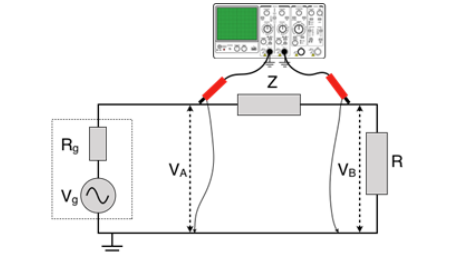
\includegraphics[width=0.5\textwidth]{grafici/circuito-rc.png}
	\caption{Circuito RC}
	\label{fig:rc_circuito}
\end{figure}
Per poter effettuare le misure abbiamo realizzato un circuito sulla breadboard come in figura~\ref{fig:rc_circuito}. In questo caso $Z$ rappresenta la capacità $C$. Per poter campionare la forma d'onda di $V_C(t)$ e $V_R(t)$ abbiamo utilizzato un oscilloscopio a cui sono state collegate due sonde. Una sonda è stata posizionata in modo tale da misurare l'andamento di $V_g(t)$, segnale sinusoidale, mentre l'altra è stata posizionata ai capi di $R$. Per misurare la caduta di potenziale ai capi della capacità $C$ abbiamo utilizzato la funzione \texttt{math} dell'oscilloscopio la quale permette di eseguire operazioni matematiche con le onde in ingresso; nel nostro caso abbiamo impostato come operazione la sottrazione fra la tensione ai capi del generatore e la tensione ai capi della resistenza in modo da ottenere la tensione ai capi della capacità, infatti:
$V_g(t) = V_C(t) + V_R(t)$, dunque $V_C(t) = V_g(t) - V_R(t)$. Nell'ipotesi in cui $R$ e $C$ fossero state scambiate di posizione all'interno del circuito, i loro ruoli si sarebbero invertiti anche all'interno della definizione della differenza restituita dall'oscilloscopio.
Come resistenza abbiamo utilizzato una cassetta di resistenze che permette di scegliere un valore di $R$ arbitrario con un errore dell'\SI{1}{\percent}. Per misurare l'ampiezza e la fase delle onde abbiamo utilizzato la funzione \texttt{math} dell'oscilloscopio: nel caso dell'ampiezza essa restituisce la distanza picco-picco, dunque il doppio dell'ampiezza di ciascuna onda, mentre per quanto riguarda la fase misura lo sfasamento temporale tra il massimo dell'onda in esame e il relativo massimo dell'onda di riferimento.

\subsection{Dati}
Per la realizzazione del circuito abbiamo impostato $R_{nota} = \SI{10.0 \pm 0.1}{k\ohm}$, in modo tale da poter considerare trascurabile sia la resistenza interna dell'oscilloscopio che del generatore.\footnote{Considerando $R_{nota} = \SI{10.0}{k\ohm}$ e $R_{osc} = \SI{1}{M\ohm}$, la resistenza effettiva dovuta al parallelo è $R'_{nota} = (R_{nota} \cdot R_{osc})/(R_{nota} + R_{osc}) \approx \SI{9901}{\ohm}$. Questa differisce da $R_{nota}$ di circa $\SI{99}{\ohm}$. L'incertezza su $R_{nota}$ è $\SI{100}{\ohm}$ (\SI{1}{\percent} di $\SI{10}{k\ohm}$). Quindi, la variazione dovuta a $R_{osc}$ è dello stesso ordine di grandezza dell'incertezza su $R_{nota}$. La resistenza $R_g \approx \SI{1}{\ohm}$ in serie introduce una variazione molto più piccola, quindi trascurabile in confronto.}
Per quanto riguarda invece la capacità inserita nel circuito, ne abbiamo misurato il valore mediante un multimetro, ricavando $C_{nota} = \SI{96 \pm 1}{nF}$.
Impostato $V_g(t)$ dal generatore, abbiamo dapprima verificato che la forma d'onda erogata coincidesse con quanto restituito dall'oscilloscopio, dopodiché abbiamo misurato l'ampiezza della tensione ai capi del generatore mediante la funzionalità picco-picco. Fissato $V_g$ (inteso come ampiezza picco-picco), abbiamo poi raccolto circa 20 valori delle due coppie $V_C - \nu$ e $V_R - \nu$, dove $V_C$ e $V_R$ indicano la distanza picco-picco per $V(t)$ ai capi della capacità e della resistenza, mentre $\nu$ indica la frequenza impostata sul generatore. Tale frequenza è stata scelta in un intorno della frequenza di taglio, stimata come $\nu_t = \frac{1}{2\pi R_{nota}C_{nota}} = \SI{165.79}{\hertz}$.
Utilizzando le medesime frequenze è stato misurato anche lo sfasamento $\Delta\phi_C$ della funzione $V_C(t)$ e $\Delta\phi_R$ di $V_R(t)$ rispetto a $V_g(t)$. Per quanto riguarda le incertezze abbiamo valutato i valori di frequenza come privi di errore, mentre abbiamo stimato l'errore sulle distanze picco-picco utilizzando la precisione dell'oscilloscopio, ossia metà dell'intervallo entro cui oscillavano i valori da esso restituiti. Per quanto riguarda le fasi\footnote{Le fasi sono state restituite dall'oscilloscopio in gradi, in tabella sono già state convertite in radianti.}, abbiamo misurato ciascun valore come media del range di oscillazione della misura stessa sull'oscilloscopio, e l'errore associato come metà ampiezza dell'oscillazione.
Ciò è riportato in tabella.
\begin{table}[htbp]
    \centering
    \begin{tabular}{|c|c|c|c|c|c|}
    \hline
    Frequenza & $V_g$ & $V_C$ & $V_R$ & $\Delta\phi_C$ & $\Delta\phi_R$ \\\hline\hline
    10 ± 0 Hz & 4.0 ± 0.4 V & 4.0 ± 0.8 V & 12.8 ± 0.4 mV & 3.11 ± 0.03 rad & 1.6 ± 0.1 rad \\
    15 ± 0 Hz & 4.0 ± 0.4 V & 4.1 ± 0.8 V & 18.0 ± 0.4 mV & 3.07 ± 0.03 rad & 1.56 ± 0.05 rad \\
    25 ± 0 Hz & 4.0 ± 0.4 V & 4.1 ± 0.8 V & 28.8 ± 0.4 mV & 3.12 ± 0.02 rad & 1.55 ± 0.02 rad \\
    50 ± 0 Hz & 4.0 ± 0.4 V & 4.1 ± 0.8 V & 57.6 ± 0.8 mV & 3.09 ± 0.03 rad & 1.58 ± 0.01 rad \\
    100 ± 0 Hz & 4.0 ± 0.4 V & 4.1 ± 0.8 V & 112 ± 2 mV & 3.09 ± 0.03 rad & 1.54 ± 0.02 rad \\
    120 ± 0 Hz & 4.0 ± 0.4 V & 4.1 ± 0.8 V & 134 ± 2 mV & 3.14 ± 0.02 rad & 1.55 ± 0.02 rad \\
    150 ± 0 Hz & 4.0 ± 0.4 V & 4.1 ± 0.8 V & 168 ± 2 mV & 3.05 ± 0.03 rad & 1.54 ± 0.02 rad \\
    200 ± 0 Hz & 4.0 ± 0.4 V & 4.0 ± 0.4 V & 228 ± 4 mV & 3.09 ± 0.03 rad & 1.52 ± 0.02 rad \\
    300 ± 0 Hz & 4.0 ± 0.4 V & 4.0 ± 0.2 V & 336 ± 2 mV & 3.04 ± 0.03 rad & 1.48 ± 0.02 rad \\
    450 ± 0 Hz & 4.0 ± 0.4 V & 4.08 ± 0.08 V & 504 ± 2 mV & 3.00 ± 0.03 rad & 1.47 ± 0.02 rad \\
    700 ± 0 Hz & 4.0 ± 0.4 V & 4.0 ± 0.4 V & 784 ± 2 mV & 2.97 ± 0.02 rad & 1.39 ± 0.02 rad \\
    1 ± 0 kHz & 4.0 ± 0.4 V & 3.96 ± 0.04 V & 1.09 ± 0.03 V & 2.86 ± 0.03 rad & 1.30 ± 0.02 rad \\
    1.5 ± 0.0 kHz & 4.0 ± 0.4 V & 3.76 ± 0.04 V & 1.58 ± 0.04 V & 2.74 ± 0.02 rad & 1.18 ± 0.02 rad \\
    2.2 ± 0.0 kHz & 4.0 ± 0.4 V & 3.48 ± 0.04 V & 2.14 ± 0.04 V & 2.60 ± 0.02 rad & 1.03 ± 0.02 rad \\
    3.2 ± 0.0 kHz & 4.0 ± 0.4 V & 3.00 ± 0.04 V & 2.70 ± 0.04 V & 2.43 ± 0.02 rad & 836 ± 20 mrad \\
    4.5 ± 0.0 kHz & 4.0 ± 0.4 V & 2.52 ± 0.04 V & 3.18 ± 0.04 V & 2.23 ± 0.02 rad & 677 ± 20 mrad \\
    6 ± 0 kHz & 4.0 ± 0.4 V & 2.12 ± 0.04 V & 3.48 ± 0.04 V & 2.09 ± 0.02 rad & 543 ± 20 mrad \\
    7.5 ± 0.0 kHz & 4.0 ± 0.4 V & 1.80 ± 0.04 V & 3.64 ± 0.04 V & 2.01 ± 0.02 rad & 452 ± 20 mrad \\
    10 ± 0 kHz & 4.0 ± 0.4 V & 1.40 ± 0.04 V & 3.80 ± 0.04 V & 1.88 ± 0.02 rad & 339 ± 20 mrad \\
    15 ± 0 kHz & 4.0 ± 0.4 V & 1.00 ± 0.04 V & 3.92 ± 0.04 V & 1.80 ± 0.02 rad & 236 ± 20 mrad \\
    20 ± 0 kHz & 4.0 ± 0.4 V & 760 ± 40 mV & 3.98 ± 0.04 V & 1.78 ± 0.02 rad & 176 ± 20 mrad \\
    30 ± 0 kHz & 4.0 ± 0.4 V & 560 ± 40 mV & 4.04 ± 0.04 V & 1.64 ± 0.02 rad & 113 ± 3 mrad \\
    \hline
    \end{tabular}
    \caption{Dati Sperimentali per il Circuito RC.}
    \label{tab:dati_sperimentali_rc}
    \end{table}

\subsection{Analisi dati}
Dopo aver calcolato le pulsazioni $\omega = 2\pi \nu$, abbiamo analizzato separatamente ampiezza e fase per valutare le funzioni di trasferimento $H_C(\omega)$ sulla capacità e $H_R(\omega)$ sulla resistenza. In entrambi i casi abbiamo considerato il rapporto della distanza picco-picco della tensione in uscita con quella della tensione in entrata, in modo tale da ottenere il rapporto tra le ampiezze.\footnote{La distanza picco-picco corrisponde al doppio dell'ampiezza; valutando il rapporto i fattori 2 però si semplificano.}
Abbiamo quindi fittato i valori così ricavati con le funzioni che descrivono l'andamento atteso della funzione di trasferimento. Più precisamente, dall'analisi circuitale e dall'applicazione del concetto di impedenza sono state ricavate le relazioni seguenti:
\begin{align}
|H_C(\omega)| = \frac{1}{\sqrt{1 + (\omega RC)^2}} \qquad & \text{,}\qquad |H_R(\omega)| = \frac{\omega RC}{\sqrt{1 + (\omega RC)^2}} \label{eq:ampiezza RC} \\
\arg H_C(\omega) = -\arctan(\omega RC) \qquad & \text{,}\qquad \arg H_R(\omega) = \frac{\pi}{2}-\arctan(\omega RC) \label{eq: fase RC}
\end{align}
Le relazioni riguardanti lo sfasamento delle funzioni di trasferimento possono considerarsi verificate a meno di multipli interi di $\pi$; ciò che è importante è infatti che $\arg H_C(\omega)$ e $\arg H_R(\omega)$ siano sfasati di $\frac{\pi}{2}$.
Quanto ricavato dai fit è osservabile nei grafici \ref{fig:funzioni_di_trasferimento_rc}.
\begin{figure}[htbp]
    \centering

    \begin{subfigure}[b]{0.495\textwidth}
        \centering
        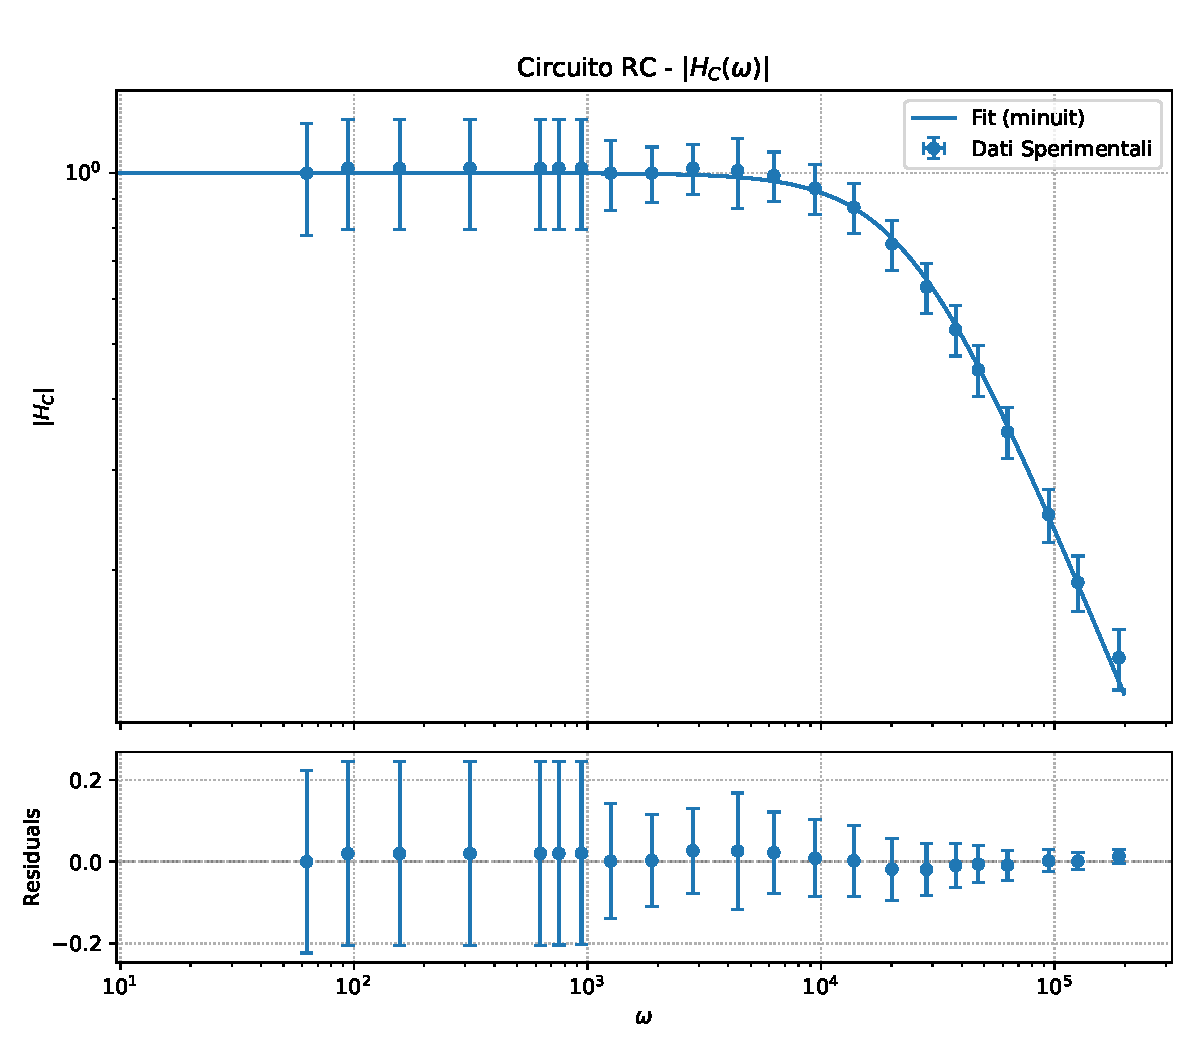
\includegraphics[width=\linewidth]{grafici/rc_hc.pdf}
        \caption{Fit modulo $|H_C(\omega)|$}
        \label{fig:rc_hc}
    \end{subfigure}
    \hfill
    \begin{subfigure}[b]{0.495\textwidth}
        \centering
        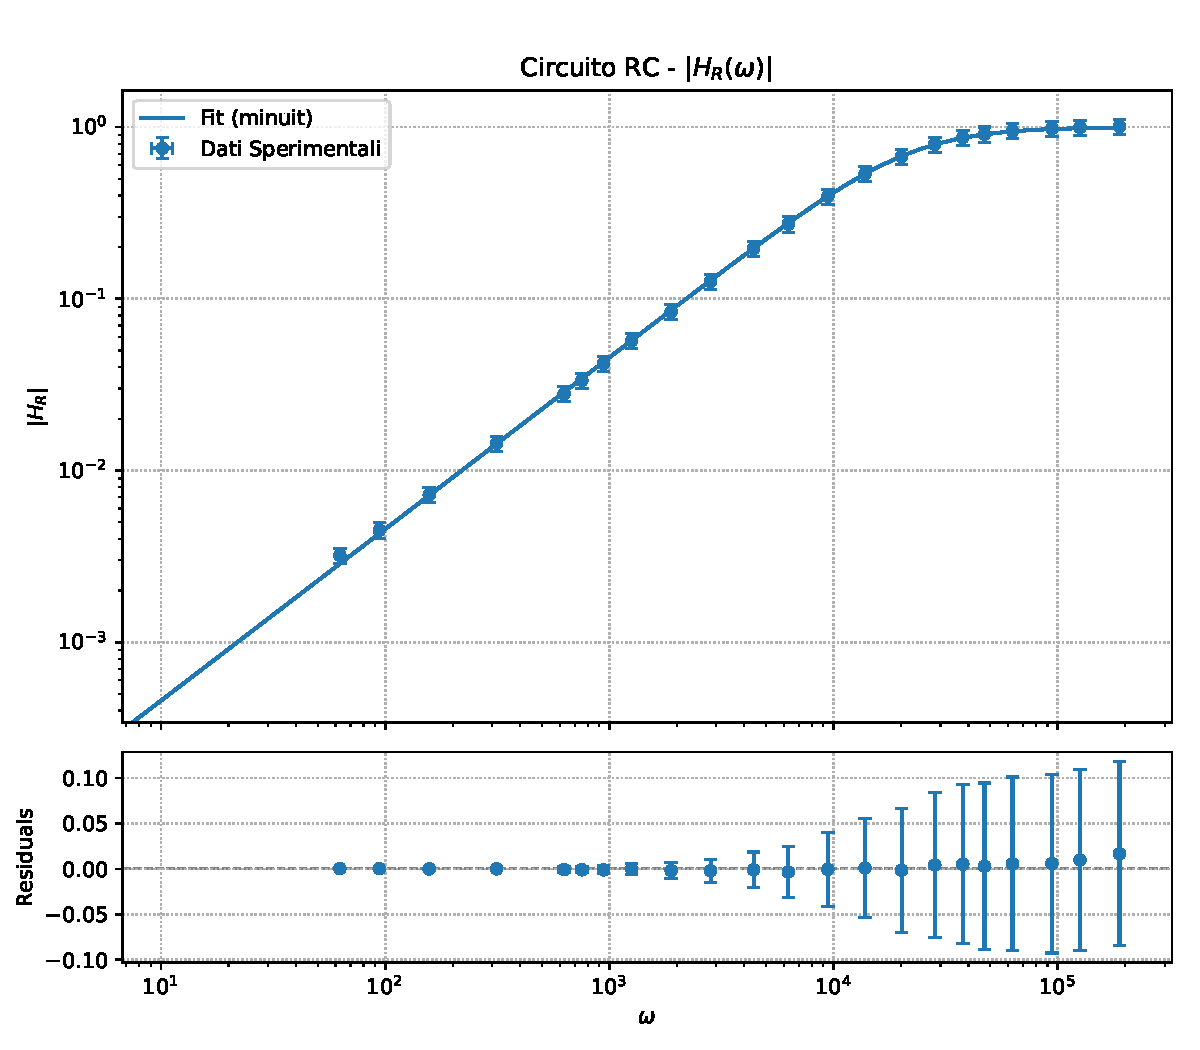
\includegraphics[width=\linewidth]{grafici/rc_hr.pdf}
        \caption{Fit modulo $|H_R(\omega)|$}
        \label{fig:rc_hr}
    \end{subfigure}

    \vspace{\baselineskip}

    \begin{subfigure}[b]{0.495\textwidth}
        \centering
        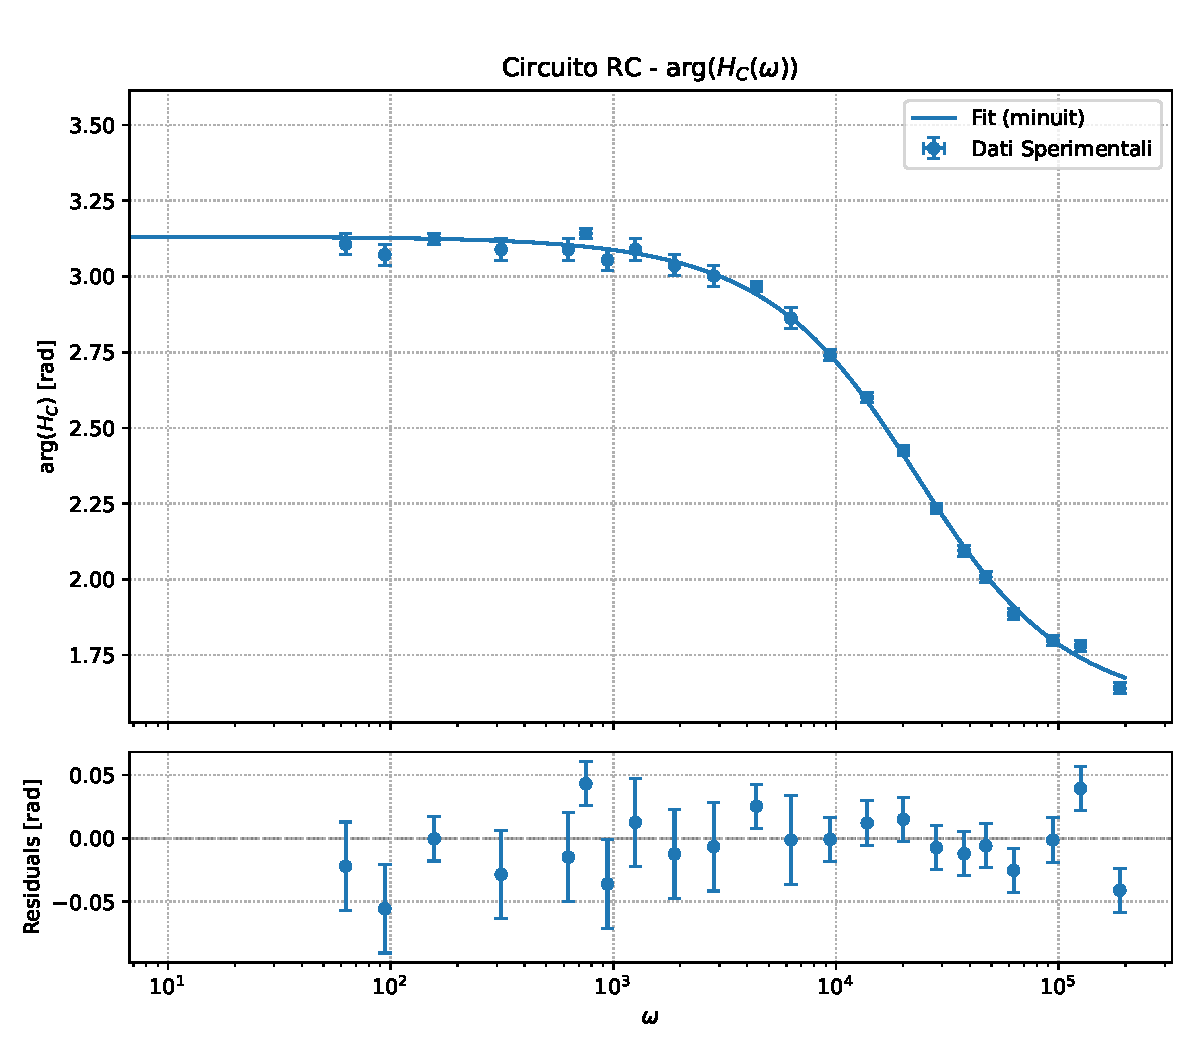
\includegraphics[width=\linewidth]{grafici/rc_fase_hc.pdf}
        \caption{Fit fase $H_C(\omega)$}
        \label{fig:rc_fase_hc}
    \end{subfigure}
    \hfill
    \begin{subfigure}[b]{0.495\textwidth}
        \centering
        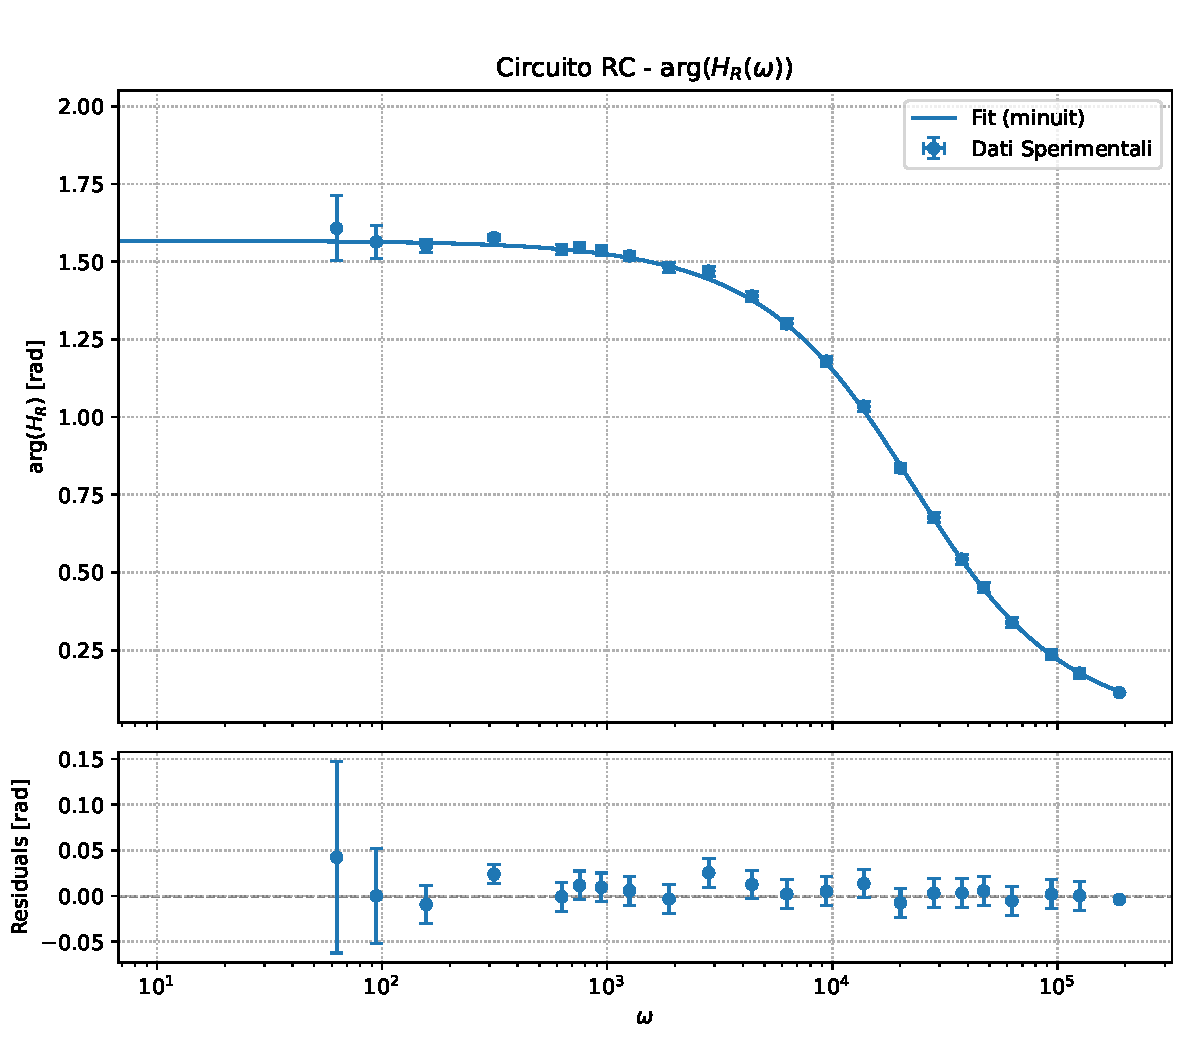
\includegraphics[width=\linewidth]{grafici/rc_fase_hr.pdf}
        \caption{Fit fase $H_R(\omega)$}
        \label{fig:rc_fase_hr}
    \end{subfigure}

    \caption{Funzioni di trasferimento RC}
    \label{fig:funzioni_di_trasferimento_rc}
\end{figure}

Come si può osservare, il circuito RC si comporta come un filtro passa-basso se valutiamo il trasferimento della tensione sulla capacità.
Infatti il modulo della funzione di trasferimento per la differenza di potenziale ai capi della capacità è prossimo a 1 per basse frequenze (e quindi basse pulsazioni) e tende a 0 per valori molto alti di $\omega$.
Nella realizzazione dei fit abbiamo fissato il parametro $R$, imponendo $R = R_{nota} = \SI{10.0 \pm 0.1}{k\ohm}$ e abbiamo ricavato i valori di $C_s$.
I valori di capacità ricavati per ciascun fit sono riportati nella tabella~\ref{tab:risultati_fit_rc}.
Tali capacità sono state utilizzate per ottenere una stima empirica del valore di $C$, calcolato mediante la media pesata, e del suo errore $\delta_{C_{media}}$, corrispondente alla deviazione standard sulla media pesata; risulta quindi $C_{media} = \SI{4.40 \pm 0.06}{nF}$.
Le capacità sono state confrontate mediante z-test; tra loro, con $z = \frac{C_1 - C_2}{\sqrt{\delta_{C_1}^2 + \delta_{C_2}^2}}$, e con $C_{att}$ (capacità attesa, presumibilmente $C_{nota}$), con $z = \frac{C_s - C_{att}}{\sqrt{\delta_{C_s}^2 + \delta_{C_{att}}^2}}$. I risultati del test di compatibilità\footnote{Le $C$ ricavate differiscono di un ordine di grandezza da $C_{nota}$, lo z-test è superfluo in questo caso.} sono visibili in seguito, nella tabella~\ref{tab:rc_compatibilita_C}.
Nella realizzazione dei fit per le fasi delle funzioni di trasferimento è stato impostato un offset, corrispondente ad una traslazione sull'asse verticale (fase). I valori di tale parametro ricavati mediante fit sono riportati in tabella~\ref{tab:risultati_fit_rc}. Il parametro $k_R$ (ricavato per il fit sulla fase di $H_R(\omega)$) risulta compatibile con una traslazione di $\frac{\pi}{2}$, come previsto dalla relazione~\eqref{eq: fase RC}. Al contrario il parametro $k_C$ (ricavato per il fit sulla fase di $H_C(\omega)$) risulta compatibile con un valore di $\pi$.
Infine è stato valutato l'accordo tra i dati sperimentali e le funzioni di fit ricavate utilizzando il test del chi quadro (tabella~\ref{tab:risultati_fit_rc}).
\begin{table}[htbp]
    \centering
    \begin{tabular}{|l|cccc|}
    \hline
    Dato & $|H_C|$ & $|H_R|$ & $\arg(H_C)$ & $\arg(H_R)$ \\\hline\hline
    $C$ & 4.14 ± 0.20 nF & 4.57 ± 0.13 nF & 4.37 ± 0.11 nF & 4.401 ± 0.081 nF \\\hline
    $k$ & --- & --- & 3.1314 ± 0.0079 rad & 1.5678 ± 0.0035 rad \\\hline
    $\chi^2$ & 1.04 & 1.48 & 28 & 13.4 \\\hline
    DoF & 21 & 21 & 20 & 20 \\\hline
    $\chi^2/\text{DoF}$ & 0.0495 & 0.0707 & 1.4 & 0.67 \\\hline
    \end{tabular}
    \caption{Risultati dei Fit per il Circuito RC.}
    \label{tab:risultati_fit_rc}
\end{table}
\begin{table}[htbp]
\centering
\begin{tabular}{|l|cccc|}
\hline
Fit Confrontato & $|H_C|$ & $|H_R|$ & $\arg(H_C)$ & $\arg(H_R)$ \\\hline\hline
$|H_C|$ & --- & \shortstack{Z=1.81 \\ \checkmark} & \shortstack{Z=0.98 \\ \checkmark} & \shortstack{Z=1.20 \\ \checkmark} \\\hline
$|H_R|$ & \shortstack{Z=1.81 \\ \checkmark} & --- & \shortstack{Z=1.19 \\ \checkmark} & \shortstack{Z=1.11 \\ \checkmark} \\\hline
$\arg(H_C)$ & \shortstack{Z=0.98 \\ \checkmark} & \shortstack{Z=1.19 \\ \checkmark} & --- & \shortstack{Z=0.25 \\ \checkmark} \\\hline
$\arg(H_R)$ & \shortstack{Z=1.20 \\ \checkmark} & \shortstack{Z=1.11 \\ \checkmark} & \shortstack{Z=0.25 \\ \checkmark} & --- \\\hline
\end{tabular}
\caption{Risultati dei test di compatibilità (Z-score e valutazione a $\alpha=0.05$) tra i valori del parametro $C$ ottenuti dai diversi fit per il circuito RC. Si assume indipendenza tra i risultati dei fit. (Z: Z-score; $\checkmark$: Compatibile; $\times$: Non Compatibile)}
\label{tab:rc_compatibilita_C}
\end{table}

\subsection{Conclusioni}
Basandoci sui risultati dei test del chi quadro (tabella~\ref{tab:risultati_fit_rc}) possiamo affermare che le leggi ricavate per il modulo e le fasi della funzione di trasferimento offrono un buon accordo con i dati sperimentali sia per quanto riguarda $H_C(\omega)$ che per quanto riguarda $H_R(\omega)$. I risultati di $C$ ottenuti dalle funzioni di trasferimento interpolate risultano essere compatibili tra di loro (tabella~\ref{tab:rc_compatibilita_C}), tuttavia essi non risultano essere compatibili con la capacità attesa $C_{nota} = \SI{96 \pm 1}{nF}$ misurata in laboratorio con il multimetro. Dal momento che i valori di $C$ determinati sperimentalmente risultano coerenti tra di loro ma in forte disaccordo con $C_{nota}$ possiamo ipotizzare di aver compiuto una misura errata del valore di quest'ultima, non avendo però raccolto informazioni rilevanti sul multimetro (utilizzato esclusivamente per la misura di $C_{nota}$) non sappiamo come giustificare esaustivamente la discrepanza.


\section{Circuito RL}
\subsection{Obiettivo}
Valutare la risposta in frequenza di un circuito RL alimentato da un generatore di segnale impostato su funzioni sinusoidali (della forma
$V_g(t) = V_{0} \cos(\omega t + \phi)$). Studiare sia l'andamento dell'ampiezza che della fase della funzione di trasferimento per la tensione ai capi della resistenza e dell'induttanza.
\subsection{Metodo}
Per poter effettuare le misure abbiamo realizzato un circuito sulla breadboard come in figura~\ref{fig:rc_circuito}. In questo caso $Z$ rappresenta l'induttanza $L$. Per poter campionare la forma d'onda di $V_L(t)$ e $V_R(t)$ abbiamo utilizzato un oscilloscopio a cui sono state collegate due sonde. Una sonda è stata posizionata in modo tale da misurare l'andamento di $V_g(t)$, mentre l'altra è stata posizionata ai capi di $R$. Come effettuato per $C$, per misurare la caduta di potenziale ai capi dell'induttanza $L$ abbiamo utilizzato la funzione \texttt{math} dell'oscilloscopio, più precisamente la differenza $V_L(t) = V_g(t) - V_R(t)$. Tale funzione ci ha anche permesso di campionare la distanza picco-picco (due volte l'ampiezza) delle varie onde e la loro fase rispetto a $V_g(t)$. Anche in questo caso la resistenza è stata scelta utilizzando la cassetta di resistenze, sulla quale è indicato un errore dell'\SI{1}{\percent} sul valore della resistenza scelta.

\subsection{Dati}
Possiamo effettuare un ragionamento analogo al precedente per quanto riguarda i valori di resistenza utilizzati, considerando trascurabili la resistenza interna dell'induttanza, dell'oscilloscopio e del generatore e deducendo quindi $R_{eq} \approx R_{nota} = \SI{10.0 \pm 0.1}{k\ohm}$. In quanto ignoto il valore dell'induttanza inserita nel circuito, non abbiamo potuto stimare la frequenza di taglio $\nu_t = \frac{R}{2\pi L}$. Abbiamo misurato la distanza picco-picco del segnale di tensione ai capi dell'induttanza e della resistenza per circa 15 valori di frequenza, al fine di campionare l'ampiezza delle funzioni di trasferimento. Per ricavarne invece la fase abbiamo osservato l'andamento dello sfasamento $\Delta\phi_L$ (di $V_L(t)$) e $\Delta\phi_R$ (di $V_R(t)$) rispetto a $V_g(t)$ in funzione della frequenza. I valori di $\nu$ impostati da generatore, e di conseguenza di $\omega = 2\pi \nu$, sono i medesimi. Come descritto per il circuito RC abbiamo considerato i valori di frequenza come privi di errore. Per determinare invece l'incertezza sull'ampiezza e lo sfasamento delle onde che descrivevano l'andamento della tensione ai capi dei vari elementi circuitali, abbiamo considerato la precisione con cui le misure venivano restituite dall'oscilloscopio. Unica eccezione consiste in quanto valutato per l'ampiezza della funzione di trasferimento sull'induttanza. In quest'ultimo caso per alte frequenze l'ampiezza di $V_L(t)$ (segnale in uscita) figurava maggiore di quella di $V_g(t)$ (segnale in entrata); evidenza sperimentale che ci ha portato ad ipotizzare che il circuito entrasse in risonanza, si comportasse cioè come circuito RLC, a causa della presenza delle capacità interne delle componenti del circuito, fino ad ora considerate trascurabili. Non potendo però confermare tale ipotesi ci siamo limitati a considerare un'incertezza maggiore sui valori della distanza picco-picco per la funzione $V_L(t)$. Quanto così ricavato è inserito in tabella~\ref{tab:dati_sperimentali_rl}.
\begin{table}[htbp]
    \centering
    \begin{tabular}{|c|c|c|c|c|c|}
    \hline
    Frequenza & $V_g$ & $V_L$ & $V_R$ & $\Delta\phi_L$ & $\Delta\phi_R$ \\\hline\hline
    5 ± 0 kHz & 4.2 ± 0.4 V & 640 ± 10 mV & 4.07 ± 0.01 V & -1.57 ± 0.03 rad & -148 ± 9 mrad \\
    7 ± 0 kHz & 4.2 ± 0.4 V & 980 ± 20 mV & 4.00 ± 0.02 V & -1.66 ± 0.03 rad & -227 ± 20 mrad \\
    10 ± 0 kHz & 4.2 ± 0.4 V & 1.36 ± 0.01 V & 4.04 ± 0.04 V & -1.76 ± 0.03 rad & -279 ± 20 mrad \\
    15 ± 0 kHz & 4.2 ± 0.4 V & 1.84 ± 0.01 V & 3.90 ± 0.02 V & -1.8 ± 0.1 rad & -436 ± 20 mrad \\
    20 ± 0 kHz & 4.2 ± 0.4 V & 2.32 ± 0.01 V & 3.74 ± 0.02 V & -2.0 ± 0.1 rad & -559 ± 20 mrad \\
    25 ± 0 kHz & 4.2 ± 0.4 V & 2.68 ± 0.04 V & 3.50 ± 0.02 V & -2.09 ± 0.02 rad & -654 ± 9 mrad \\
    50 ± 0 kHz & 4.2 ± 0.4 V & 3.80 ± 0.04 V & 2.50 ± 0.02 V & -2.48 ± 0.03 rad & -1.08 ± 0.02 rad \\
    75 ± 0 kHz & 4.2 ± 0.4 V & 4.24 ± 0.04 V & 1.80 ± 0.02 V & -2.71 ± 0.02 rad & -1.34 ± 0.03 rad \\
    100 ± 0 kHz & 4.2 ± 0.4 V & 4.32 ± 0.08 V & 1.34 ± 0.02 V & -2.83 ± 0.02 rad & -1.52 ± 0.03 rad \\
    125 ± 0 kHz & 4.2 ± 0.4 V & 4.40 ± 0.08 V & 980 ± 20 mV & -2.91 ± 0.03 rad & -1.66 ± 0.07 rad \\
    150 ± 0 kHz & 4.2 ± 0.4 V & 4.40 ± 0.08 V & 740 ± 20 mV & -2.98 ± 0.02 rad & -1.76 ± 0.09 rad \\
    180 ± 0 kHz & 4.2 ± 0.4 V & 4.40 ± 0.08 V & 520 ± 20 mV & -3.04 ± 0.02 rad & -1.87 ± 0.09 rad \\
    200 ± 0 kHz & 4.2 ± 0.4 V & 4.32 ± 0.04 V & 400 ± 40 mV & -3.07 ± 0.02 rad & -2.02 ± 0.09 rad \\
    225 ± 0 kHz & 4.2 ± 0.4 V & 4.24 ± 0.04 V & 184 ± 2 mV & -3.12 ± 0.02 rad & -2.11 ± 0.09 rad \\
    250 ± 0 kHz & 4.2 ± 0.4 V & 4.16 ± 0.04 V & 92 ± 4 mV & -3.14 ± 0.02 rad & -2.13 ± 0.09 rad \\
    \hline
    \end{tabular}
    \caption{Dati Sperimentali per il Circuito RL.}
    \label{tab:dati_sperimentali_rl}
    \end{table}

\subsection{Analisi dati}
Abbiamo quindi proceduto allo studio delle funzioni di trasferimento $H_L(\omega)$, la quale indica come la tensione fornita dal generatore si "trasferisce" sull'induttanza, e $H_R(\omega)$, la quale descrive invece come varia la tensione ai capi della resistenza. In entrambi i casi, per valutare il modulo della funzione di trasferimento, abbiamo considerato il rapporto della distanza picco-picco della tensione in uscita con quella della tensione in entrata. Per quanto riguarda invece le fasi, il fit ha preso in considerazione direttamente i valori di $\Delta\phi$ riportati nella tabella~\ref{tab:dati_sperimentali_rl}.
L'andamento di ampiezze e fasi di $H(\omega)$ dipende dalla pulsazione $\omega$ secondo le relazioni:
\begin{align}
	 |H_L(\omega)| = \frac{\omega L}{\sqrt{R^2 + (\omega L)^2}} \qquad & \text{,}\qquad |H_R(\omega)| = \frac{R}{\sqrt{R^2 + (\omega L)^2}} \label{eq:ampiezza RL} \\
	 \arg H_L(\omega) = \frac{\pi}{2} - \arctan\left(\frac{\omega L}{R}\right) \qquad & \text{,}\qquad \arg H_R(\omega) = -\arctan\left(\frac{\omega L}{R}\right) \label{eq:fasi RL}
\end{align}
Le relazioni riguardanti lo sfasamento delle funzioni di trasferimento possono considerarsi verificate a meno di multipli interi di $\pi$; ossia deve risultare che $\arg H_L(\omega)$ e $\arg H_R(\omega)$ siano sfasati di $\frac{\pi}{2}$. A ragione di ciò, come effettuato per il circuito RC, abbiamo realizzato i fit per gli sfasamenti valutando anche la presenza di un offset, indicato con $k$ ($k_L$ e $k_R$ riportati in tabella~\ref{tab:risultati_rl}).
I risultati del fit effettuato sono riassunti nei grafici~\ref{fig:funzioni_trasferimento_rl}.
\begin{figure}[htbp]
    \centering
    \begin{subfigure}[b]{0.495\textwidth}
        \centering
        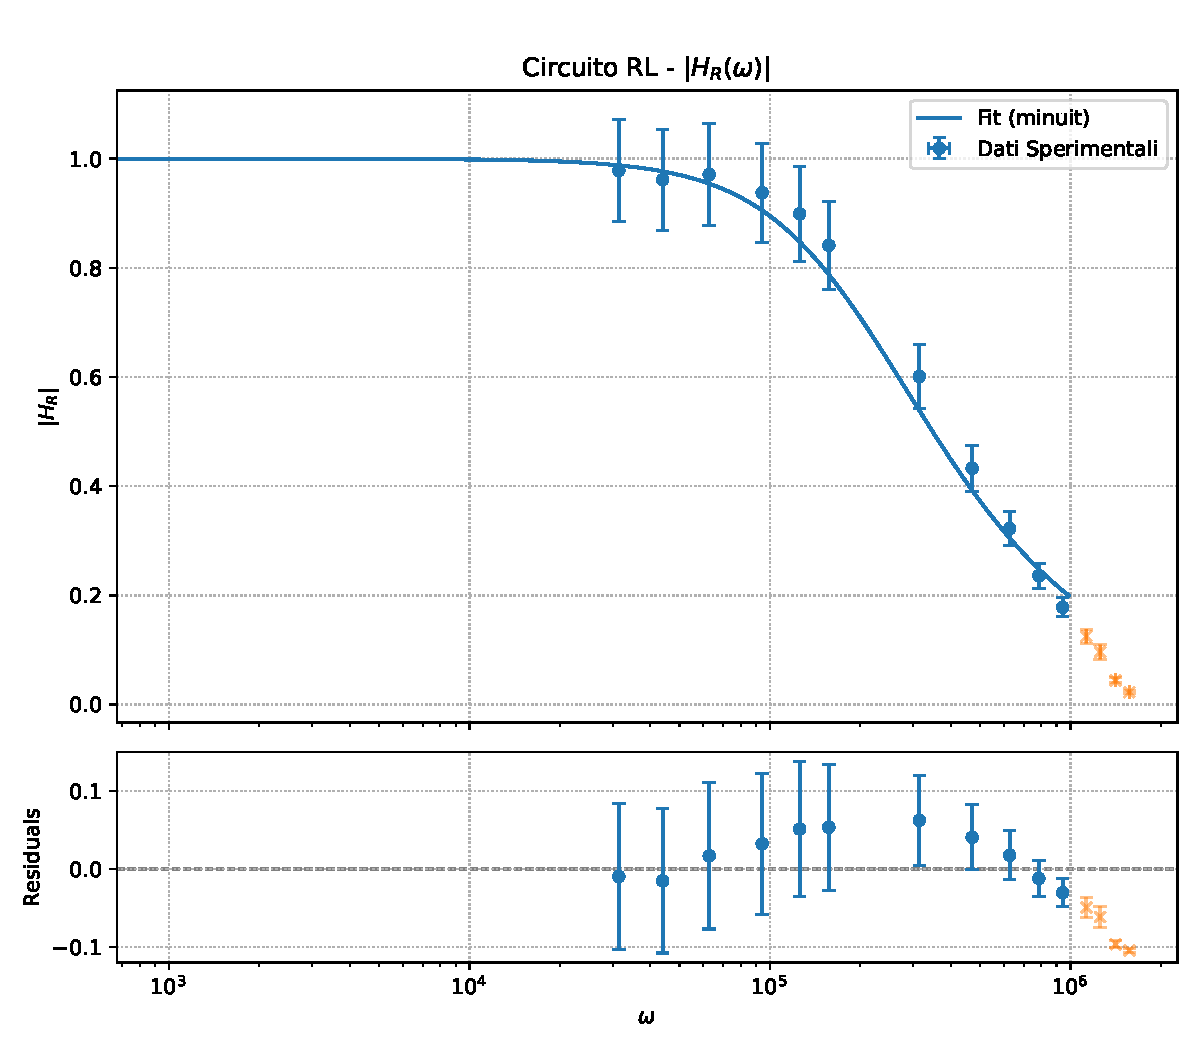
\includegraphics[width=\linewidth]{grafici/rl_hr.pdf}
        \caption{Fit modulo $|H_R(\omega)|$}
        \label{fig:rl_hr}
    \end{subfigure}
    \hfill
    \begin{subfigure}[b]{0.495\textwidth}
        \centering
        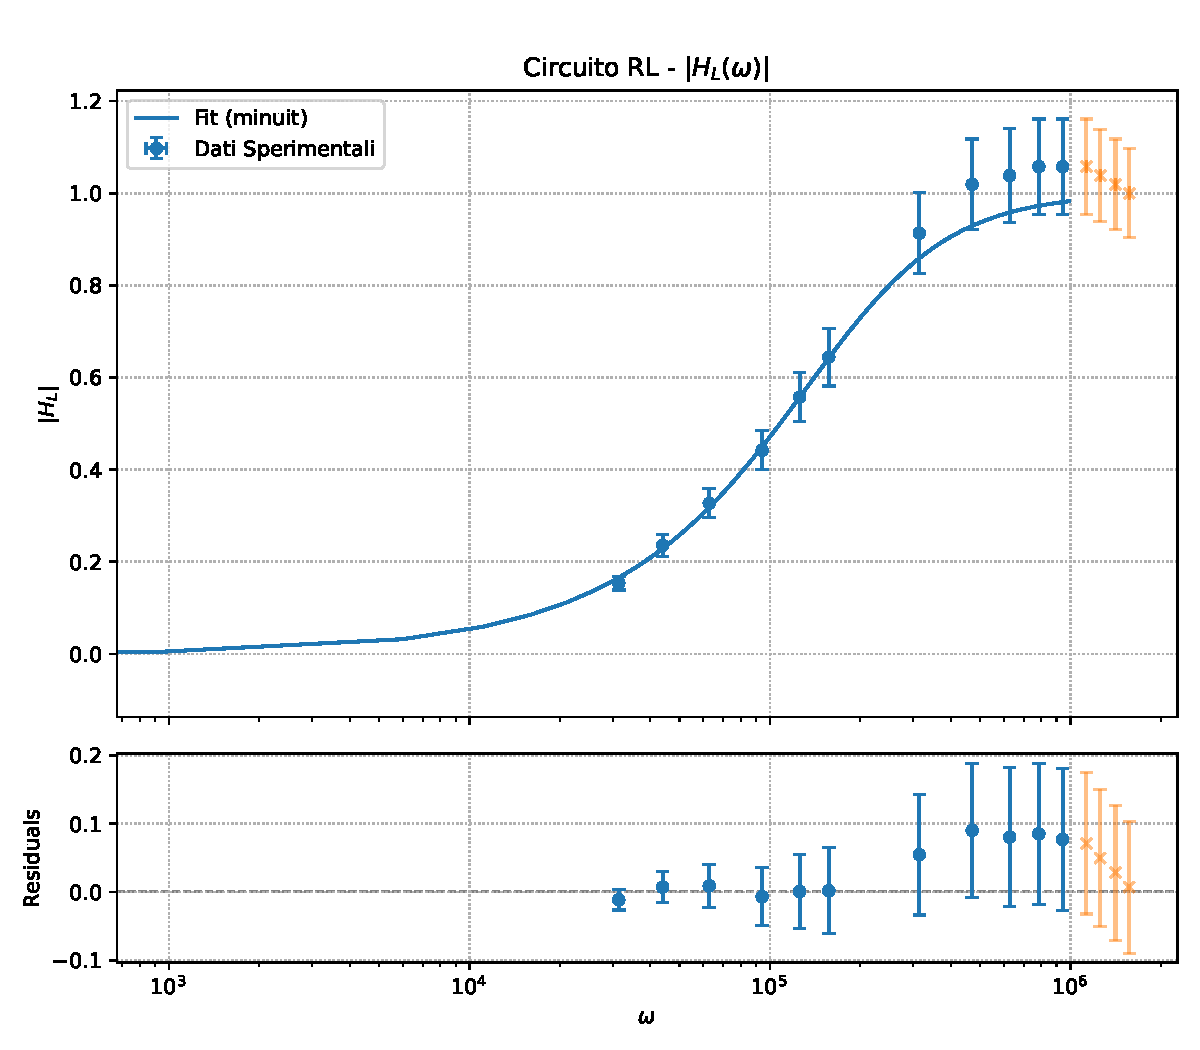
\includegraphics[width=\linewidth]{grafici/rl_hl.pdf}
        \caption{Fit modulo $|H_L(\omega)|$}
        \label{fig:rl_hl}
    \end{subfigure}

    \vspace{\baselineskip}

    \begin{subfigure}[b]{0.495\textwidth}
        \centering
        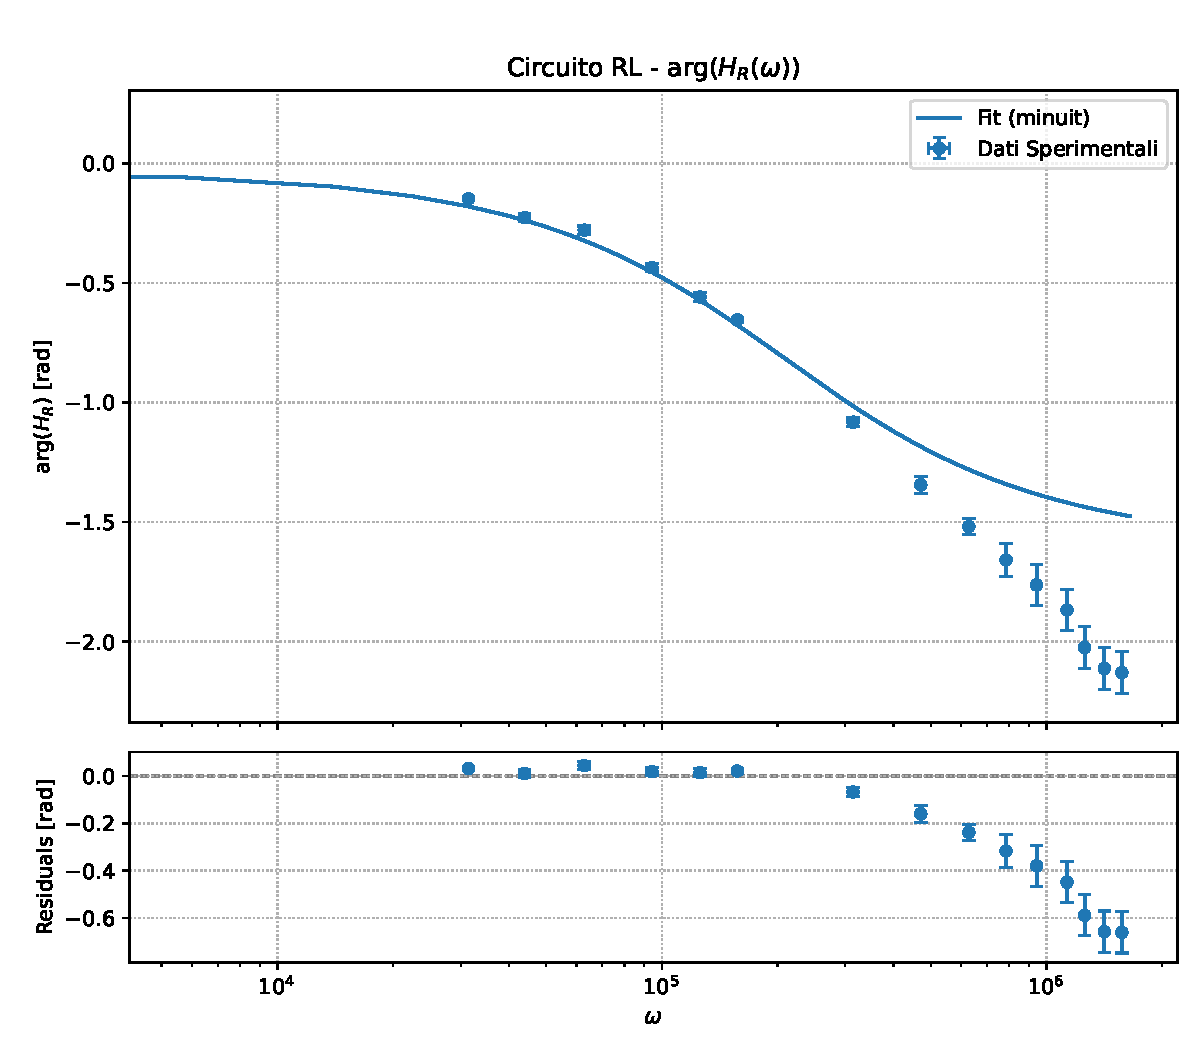
\includegraphics[width=\linewidth]{grafici/rl_fase_hr.pdf}
        \caption{Fit fase $\arg(H_R(\omega))$}
        \label{fig:rl_fase_hr}
    \end{subfigure}
    \hfill
    \begin{subfigure}[b]{0.495\textwidth}
        \centering
        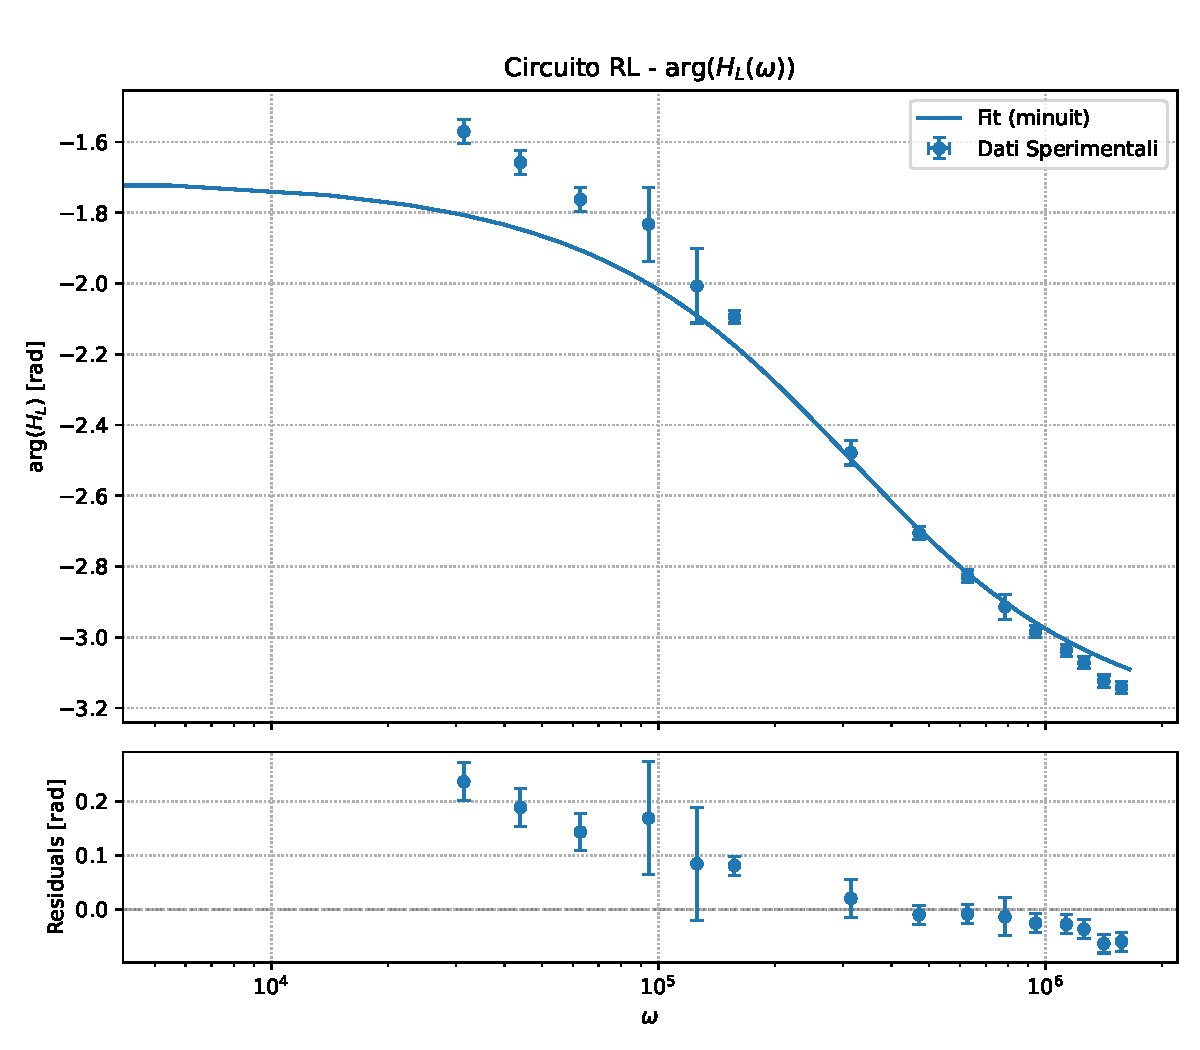
\includegraphics[width=\linewidth]{grafici/rl_fase_hl.pdf}
        \caption{Fit fase $\arg(H_L(\omega))$}
        \label{fig:rl_fase_hl}
    \end{subfigure}

    \caption{Funzioni di trasferimento RL.}
    \label{fig:funzioni_trasferimento_rl}
\end{figure}

Essi sono stati utilizzati per effettuare il test del chi quadro, atto a valutare la bontà del fit, i cui esiti sono raccolti in tabella~\ref{tab:risultati_rl}.
\begin{table}[htbp]
    \centering
    \begin{tabular}{|l|cccc|}
    \hline
    Dato & $|H_R|$ & $|H_L|$ & $\arg(H_R)$ & $\arg(H_L)$ \\\hline\hline
    $L$ & 49.8 ± 2.3 mH & 53.4 ± 2.5 mH & 47.9 ± 1.3 mH & 32.3 ± 1.3 mH \\\hline
    $k$ & --- & --- & ($-30 \pm 10)10^{-3}$  & -1.705 ± 0.013 \\\hline
    $\chi^2$ & 6.63 & 3.86 & 335 & 151 \\\hline
    DoF & 10 & 10 & 13 & 13 \\\hline
    $\chi^2/\text{DoF}$ & 0.663 & 0.386 & 25.7 & 11.6 \\\hline
    \end{tabular}
    \caption{Risultati dei Fit per il Circuito RL.}
    \label{tab:risultati_rl}
\end{table}
\begin{table}[htbp]
\centering
\begin{tabular}{|l|cccc|}
\hline
Fit Confrontato & {$|H_R|$} & {$|H_L|$} & {$\arg(H_R)$} & {$\arg(H_L)$} \\\hline\hline
$|H_R|$ & --- & \shortstack{Z=1.05 \\ \checkmark} & \shortstack{Z=0.69 \\ \checkmark} & \shortstack{Z=6.53 \\ $\times$} \\\hline
$|H_L|$ & \shortstack{Z=1.05 \\ \checkmark} & --- & \shortstack{Z=1.94 \\ \checkmark} & \shortstack{Z=7.52 \\ $\times$} \\\hline
$\arg(H_R)$ & \shortstack{Z=0.69 \\ \checkmark} & \shortstack{Z=1.94 \\ \checkmark} & --- & \shortstack{Z=8.34 \\ $\times$} \\\hline
$\arg(H_L)$ & \shortstack{Z=6.53 \\ $\times$} & \shortstack{Z=7.52 \\ $\times$} & \shortstack{Z=8.34 \\ $\times$} & --- \\\hline
\end{tabular}
\caption{Risultati dei test di compatibilità (Z-score e valutazione a $\alpha=0.05$) tra i valori del parametro $L$ ottenuti dai diversi fit per il circuito RL. Si assume indipendenza tra i risultati dei fit. (Z: Z-score; $\checkmark$: Compatibile; $\times$: Non Compatibile)}
\label{tab:rl_compatibilita_L}
\end{table}
Possiamo osservare come il circuito RL funzioni da filtro passa-alto per il trasferimento sull'induttanza: le armoniche ad alta frequenza passano infatti inalterate, con $|H_L(\omega)|$ che tende asintoticamente ad 1, mentre le armoniche a bassa frequenza vengono annullate, il modulo della funzione di trasferimento su $L$ diminuisce al diminuire della pulsazione (cioè della frequenza). Dall'osservazione dei grafici \ref{fig:funzioni_trasferimento_rl} è possibile osservare come il fit sia inizialmente buono per $\omega$ basse e poi si discosti dai dati raccolti per $\omega$ alte. Ciò è imputabile al fatto che l'oscilloscopio (o l'induttore stesso) introduce una capacità parassita non trascurabile, che va ad aggiungersi al circuito RL. Considerando l'impedenza totale del circuito, se la capacità parassita $C_p$ è in parallelo alla serie RL, vale la relazione: $Z_{eq} = \frac{1}{\frac{1}{R+j\omega L}+j\omega C_p}$. Per $\omega$ basse, il termine $j\omega C_p$ è piccolo, quindi $1/(j\omega C_p)$ è grande, e $Z_{eq} \approx R+j\omega L$, cioè il circuito si comporta come un circuito RL puro e le formule \ref{eq:ampiezza RL} e \ref{eq:fasi RL} sono valide. Quando invece si hanno $\omega$ elevate, l'effetto di $C_p$ non è più trascurabile e il circuito non si comporta più come un circuito composto esclusivamente da una resistenza ed un'induttanza in serie: bisogna tenere conto anche della presenza di una capacità $C_p$. Per tale motivo sono state ripetute le interpolazioni dei dati scartando i punti a frequenze più alte, ovvero per $\omega>10^6 rad/s$.


\subsection {Conclusione}
Basandoci sui dati ottenuti mediante il test del chi quadro (tabella~\ref{tab:risultati_rl}), possiamo affermare che le leggi attese per i moduli delle funzioni di trasferimento $H_R(\omega)$ e $H_L(\omega)$ offrono un buon accordo con i dati sperimentali (valori di $\chi^2/\text{DoF}$ inferiori a 1) nel momento in cui vengono escluse le misure effettuate a $\omega>10^6 rad/s$. Al contrario, per le fasi di tali funzioni, l'accordo non è buono (valori di $\chi^2/\text{DoF}$ elevati). Anche dopo il taglio effettuato per frequenze alte, le leggi che descrivono le fasi delle funzioni di trasferimento non rappresentano delle buone interpolazioni né per $H_L(\omega)$ né per $H_R(\omega)$. Le discrepanze nelle fasi RL, evidenziate dagli alti valori di $\chi^2/\text{DoF}$, sono probabilmente dovute agli stessi effetti capacitivi parassiti che influenzano le misure di ampiezza ad alte frequenze. La fase di un circuito è particolarmente sensibile a tali elementi parassiti, che introducono poli e zeri aggiuntivi nella funzione di trasferimento reale, rendendo inadeguato il modello teorico semplificato RL a descrivere la fase, specialmente all'avvicinarsi della frequenza di auto-risonanza dell'induttore.
Inoltre è possibile osservare come $k_R - k_L$ non risulti compatibile con una differenza di $\frac{\pi}{2}$ (considerando i valori di $k$ dalla tabella~\ref{tab:risultati_rl} e le formule teoriche per le fasi).
I valori di $L$ ottenuti dalle interpolazioni finali (ovvero scartando gli ultimi punti) non risultano essere globalmente compatibili (tabella~\ref{tab:rl_compatibilita_L}), nonostante alcune coppie di valori di $L$ mostrino accordo fra di loro. Il valore di $L$ è stato stimato comunque come la media dei valori ottenuti dai fit statisticamente validi, ossia quelli sui moduli, e corrisponde a $L_{media} = \SI{51 \pm 2}{mH}$.


\section{Circuito RLC}
\subsection{Obiettivo}
Valutare la risposta in frequenza di un circuito RLC alimentato da un generatore di segnale impostato su funzioni sinusoidali. Calcolare e studiare la funzione di trasferimento $H(\omega)$ per la tensione ai capi della resistenza, dell'induttanza e della capacità. Valutarne cioè sia l’andamento dell’ampiezza, che della fase, rispetto al segnale in entrata $V_g(t) = V_{0} \cos(\omega t + \phi)$.

\subsection{Metodo}
\begin{figure}[htbp]
	\centering
	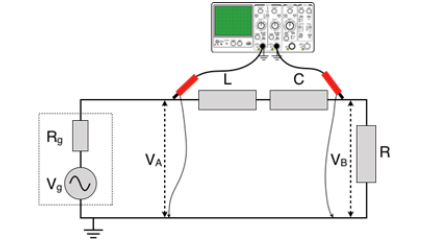
\includegraphics[width=0.5\textwidth]{grafici/circuito-rlc.png}
	\caption{Circuito RLC}
	\label{fig:rlc_circuito}
\end{figure}
Innanzitutto abbiamo ricostruito il circuito rappresentato schematicamente in figura~\ref{fig:rlc_circuito}; per farlo abbiamo collegato in serie induttore, capacitore e resistore (rappresentato dalla cassetta di resistenze). Abbiamo quindi utilizzato l'oscilloscopio per visualizzare l'andamento della tensione. Le sonde collegate all'oscilloscopio sono state collegate l'una in parallelo con il generatore, così da misurare $V_g$, e l'altra dapprima ai capi di $R$ (per misurare $V_R$), poi ai capi di $C + R$ (per misurare $V_{C+R}$), e infine ai capi di $L + R$ (per misurare $V_{L+R}$). Mentre la prima configurazione utilizzata ci ha permesso di misurare direttamente la caduta di potenziale $V_R$ ai capi della resistenza, le altre due sono state sfruttate in combinazione con la funzione \texttt{math} dell'oscilloscopio, tramite cui abbiamo misurato $V_L = V_g - V_{R+C}$ (nota: $V_g = V_L + V_R + V_C$, quindi $V_L = V_g - (V_R+V_C)$) e $V_C = V_g - V_{R+L}$ (quindi $V_C = V_g - (V_R+V_L)$).
Anche in questo caso per misurare l'ampiezza e la fase delle tensioni $V(t)$ al variare della frequenza $\nu$ impostata sul generatore, abbiamo utilizzato la funzione \texttt{math} dell'oscilloscopio: essa restituisce la distanza picco-picco, dunque il doppio dell'ampiezza, e lo sfasamento temporale tra il massimo dell'onda in esame e il massimo più vicino di $V_g(t)$. Non siamo stati però in grado di campionare l'andamento della fase per $V_L$ e $V_C$, a causa della discontinuità e dell'incertezza dei valori restituiti dall'oscilloscopio.
Tutte le misurazioni sono state effettuate impostando sulla cassetta di resistenze un valore di $R$ che determinava l'instaurarsi di un regime sovrasmorzato; ciò è stato osservato variando la forma del segnale da sinusoidale a onda quadra e valutando quanto restituito dall'oscilloscopio sulla base dell'esperienza di laboratorio precedente.

\subsection{Dati}
In quanto sono state utilizzate tre configurazioni di misura differenti, abbiamo ottenuto per la tensione ai capi della resistenza, dell'induttanza e della capacità valori dipendenti da frequenze tra loro differenti. Indicativamente si sono scelte frequenze comprese tra qualche decina e qualche centinaia di migliaia di \si{\hertz}. Inoltre è stato fondamentale osservare che al variare della frequenza impostata dal generatore, l'oscilloscopio registrava leggere variazioni della distanza picco-picco della tensione in entrata $V_g$, seppur l'ampiezza di quest'ultima non venisse variata. Abbiamo quindi appuntato queste variazioni così da tenerne conto nel calcolare i rapporti $V_L/V_g$, $V_C/V_g$ e $V_R/V_g$, ossia i moduli delle funzioni di trasferimento. Nelle tabelle~\ref{tab:dati_rlc_hr}, \ref{tab:dati_rlc_hl}, \ref{tab:dati_rlc_hc} sono riportati i valori delle distanza picco-picco per la tensione $V_g$, $V_L$, $V_C$ e $V_R$ e dello sfasamento $\Delta\phi_R$ (di $V_R(t)$) rispetto a $V_g(t)$ e i relativi errori, in funzione della frequenza $\nu$. Per quanto riguarda la stima delle incertezze abbiamo osservato gli intervalli entro cui l'oscilloscopio restituiva i valori delle distanze picco-picco e degli sfasamenti.
\begin{table}[htbp]
\centering
\begin{tabular}{|c|c|c|c|}
\hline
Frequenza & $V_g$ & $V_R$ & $\Delta\phi_R$ \\\hline\hline
100 ± 0 Hz & 4.16 ± 0.04 V & 256 ± 4 mV & 1.48 ± 0.03 rad \\
500 ± 0 Hz & 4.16 ± 0.04 V & 1.16 ± 0.02 V & 1.27 ± 0.02 rad \\
1 ± 0 kHz & 4.16 ± 0.04 V & 2.10 ± 0.04 V & 1.06 ± 0.02 rad \\
2 ± 0 kHz & 4.16 ± 0.04 V & 3.24 ± 0.04 V & 663 ± 50 mrad \\
3 ± 0 kHz & 4.16 ± 0.04 V & 3.76 ± 0.04 V & 489 ± 20 mrad \\
4 ± 0 kHz & 4.16 ± 0.04 V & 3.92 ± 0.04 V & 279 ± 20 mrad \\
6 ± 0 kHz & 4.16 ± 0.04 V & 4.08 ± 0.04 V & 113 ± 20 mrad \\
8 ± 0 kHz & 4.20 ± 0.04 V & 4.20 ± 0.08 V & 35 ± 30 mrad \\
10 ± 0 kHz & 4.32 ± 0.04 V & 4.36 ± 0.04 V & -70 ± 30 mrad \\
14 ± 0 kHz & 4.32 ± 0.04 V & 4.32 ± 0.04 V & -227 ± 20 mrad \\
18 ± 0 kHz & 4.16 ± 0.04 V & 4.08 ± 0.04 V & -332 ± 20 mrad \\
25 ± 0 kHz & 4.32 ± 0.04 V & 3.96 ± 0.04 V & -524 ± 30 mrad \\
30 ± 0 kHz & 4.32 ± 0.04 V & 3.80 ± 0.04 V & -611 ± 30 mrad \\
40 ± 0 kHz & 4.32 ± 0.04 V & 3.40 ± 0.04 V & -820 ± 30 mrad \\
50 ± 0 kHz & 4.32 ± 0.04 V & 3.04 ± 0.04 V & -977 ± 30 mrad \\
65 ± 0 kHz & 4.32 ± 0.04 V & 2.60 ± 0.04 V & -1.19 ± 0.07 rad \\
80 ± 0 kHz & 4.32 ± 0.04 V & 2.12 ± 0.04 V & -1.31 ± 0.09 rad \\
100 ± 0 kHz & 4.36 ± 0.04 V & 1.72 ± 0.04 V & -1.45 ± 0.02 rad \\
120 ± 0 kHz & 4.36 ± 0.04 V & 1.22 ± 0.02 V & -1.66 ± 0.05 rad \\
150 ± 0 kHz & 4.36 ± 0.04 V & 1.00 ± 0.04 V & -1.83 ± 0.09 rad \\
200 ± 0 kHz & 4.36 ± 0.04 V & 440 ± 40 mV & -2.02 ± 0.07 rad \\
240 ± 0 kHz & 4.36 ± 0.04 V & 220 ± 20 mV & -2.15 ± 0.09 rad \\
270 ± 0 kHz & 4.16 ± 0.04 V & 57.6 ± 0.8 mV & -2.18 ± 0.02 rad \\
\hline
\end{tabular}
\caption{Dati Sperimentali per $H_R(\omega)$ nel Circuito RLC.}
\label{tab:dati_rlc_hr}
\end{table}

\begin{table}[htbp]
\centering
\begin{tabular}{|c|c|c|}
\hline
Frequenza & $V_g$ & $V_L$ \\\hline\hline
500 ± 0 Hz & 4.12 ± 0.04 V & 280 ± 40 mV \\
1 ± 0 kHz & 4.16 ± 0.04 V & 280 ± 40 mV \\
2 ± 0 kHz & 4.12 ± 0.04 V & 360 ± 40 mV \\
5 ± 0 kHz & 4.12 ± 0.04 V & 680 ± 40 mV \\
8 ± 0 kHz & 4.16 ± 0.04 V & 960 ± 40 mV \\
10 ± 0 kHz & 4.32 ± 0.04 V & 1.40 ± 0.04 V \\
15 ± 0 kHz & 4.32 ± 0.04 V & 1.88 ± 0.04 V \\
20 ± 0 kHz & 4.32 ± 0.04 V & 2.28 ± 0.04 V \\
25 ± 0 kHz & 4.32 ± 0.04 V & 2.68 ± 0.04 V \\
30 ± 0 kHz & 4.32 ± 0.04 V & 3.00 ± 0.04 V \\
40 ± 0 kHz & 4.32 ± 0.04 V & 3.56 ± 0.04 V \\
50 ± 0 kHz & 4.32 ± 0.04 V & 3.96 ± 0.04 V \\
60 ± 0 kHz & 4.32 ± 0.04 V & 4.20 ± 0.04 V \\
70 ± 0 kHz & 4.32 ± 0.04 V & 4.36 ± 0.04 V \\
80 ± 0 kHz & 4.36 ± 0.04 V & 4.5 ± 0.2 V \\
100 ± 0 kHz & 4.36 ± 0.04 V & 4.60 ± 0.04 V \\
150 ± 0 kHz & 4.36 ± 0.04 V & 4.72 ± 0.04 V \\
200 ± 0 kHz & 4.36 ± 0.04 V & 4.60 ± 0.04 V \\
250 ± 0 kHz & 4.36 ± 0.04 V & 4.44 ± 0.02 V \\
300 ± 0 kHz & 4.36 ± 0.04 V & 4.40 ± 0.04 V \\
350 ± 0 kHz & 4.36 ± 0.04 V & 4.28 ± 0.04 V \\
\hline
\end{tabular}
\caption{Dati Sperimentali per $H_L(\omega)$ nel Circuito RLC.}
\label{tab:dati_rlc_hl}
\end{table}

\begin{table}[htbp]
\centering
\begin{tabular}{|c|c|c|}
\hline
Frequenza & $V_g$ & $V_C$ \\\hline\hline
0.04 ± 0.00 kHz & 4.12 ± 0.04 V & 4.20 ± 0.04 V \\
0.1 ± 0.0 kHz & 4.12 ± 0.04 V & 4.20 ± 0.04 V \\
0.5 ± 0.0 kHz & 4.16 ± 0.04 V & 4.00 ± 0.08 V \\
0.8 ± 0.0 kHz & 4.08 ± 0.04 V & 3.80 ± 0.04 V \\
1 ± 0 kHz & 4.08 ± 0.04 V & 3.64 ± 0.04 V \\
1.5 ± 0.0 kHz & 4.08 ± 0.04 V & 3.24 ± 0.04 V \\
2 ± 0 kHz & 4.08 ± 0.04 V & 2.84 ± 0.04 V \\
2.5 ± 0.0 kHz & 4.08 ± 0.04 V & 2.52 ± 0.04 V \\
3 ± 0 kHz & 4.08 ± 0.04 V & 2.20 ± 0.04 V \\
3.5 ± 0.0 kHz & 4.08 ± 0.04 V & 2.00 ± 0.04 V \\
4 ± 0 kHz & 4.08 ± 0.04 V & 1.84 ± 0.04 V \\
5 ± 0 kHz & 4.08 ± 0.04 V & 1.52 ± 0.04 V \\
6 ± 0 kHz & 4.08 ± 0.04 V & 1.36 ± 0.08 V \\
7 ± 0 kHz & 4.32 ± 0.04 V & 1.44 ± 0.04 V \\
9 ± 0 kHz & 4.28 ± 0.04 V & 1.24 ± 0.08 V \\
12 ± 0 kHz & 4.28 ± 0.04 V & 1.00 ± 0.04 V \\
16 ± 0 kHz & 4.28 ± 0.04 V & 800 ± 40 mV \\
22 ± 0 kHz & 4.32 ± 0.04 V & 760 ± 40 mV \\
30 ± 0 kHz & 4.32 ± 0.04 V & 720 ± 80 mV \\
40 ± 0 kHz & 4.28 ± 0.04 V & 600 ± 40 mV \\
70 ± 0 kHz & 4.28 ± 0.04 V & 500 ± 80 mV \\
100 ± 0 kHz & 4.32 ± 0.04 V & 500 ± 80 mV \\
\hline
\end{tabular}
\caption{Dati Sperimentali per $H_C(\omega)$ nel Circuito RLC.}
\label{tab:dati_rlc_hc}
\end{table}

\subsection{Analisi dati}
A partire dai dati sperimentali abbiamo ricavato la pulsazione $\omega = 2\pi \nu$ e le ampiezze delle funzioni di trasferimento dalle relazioni $|H_R(\omega)| = \frac{V_R}{V_g}$, $|H_L(\omega)| = \frac{V_L}{V_g}$ e $|H_C(\omega)| = \frac{V_C}{V_g}$.
Per tali grandezze è stato eseguito un fit utilizzando la forma funzionale delle funzioni di trasferimento attese, sia per l'ampiezza che per lo sfasamento (ove disponibile). In seguito riportiamo le relazioni ricavate a partire dall'analisi circuitale del circuito RLC e dalla rappresentazione delle sue caratteristiche mediante coefficienti complessi (impedenze).
\begin{align}
	 |H_L(\omega)| = \frac{\omega L}{\sqrt{R^2 + \left(\omega L-\frac{1}{\omega C}\right)^2}} \qquad & \text{,}\qquad |H_C(\omega)| = \frac{1/(\omega C)}{\sqrt{R^2 + \left(\omega L-\frac{1}{\omega C}\right)^2}} \label{eq:ampiezze VL, Vc RLC} \\
	 |H_R(\omega)| = \frac{R}{\sqrt{R^2 + \left(\omega L-\frac{1}{\omega C}\right)^2}} \qquad & \text{,}\qquad \arg H_R(\omega) = -\arctan\left(\frac{\omega L -\frac{1}{\omega C}}{R}\right) \label{eq:Vr_RLC}
\end{align}
Per ogni fit abbiamo considerato come noto il valore della resistenza equivalente del circuito $R_{eq} \approx R_{nota} = \SI{10.0 \pm 0.1}{k\ohm}$, approssimabile appunto alla resistenza impostata manualmente in quanto rispetto ad essa la resistenza interna dell'oscilloscopio (collegata in parallelo), del generatore e dell'induttanza (collegate in serie) risultavano trascurabili. L'esito dei fit realizzati è visualizzabile nei grafici~\ref{fig:funzioni_trasferimento_rlc}.
\begin{figure}[htbp]
    \centering

    \begin{subfigure}[b]{0.495\textwidth}
        \centering
        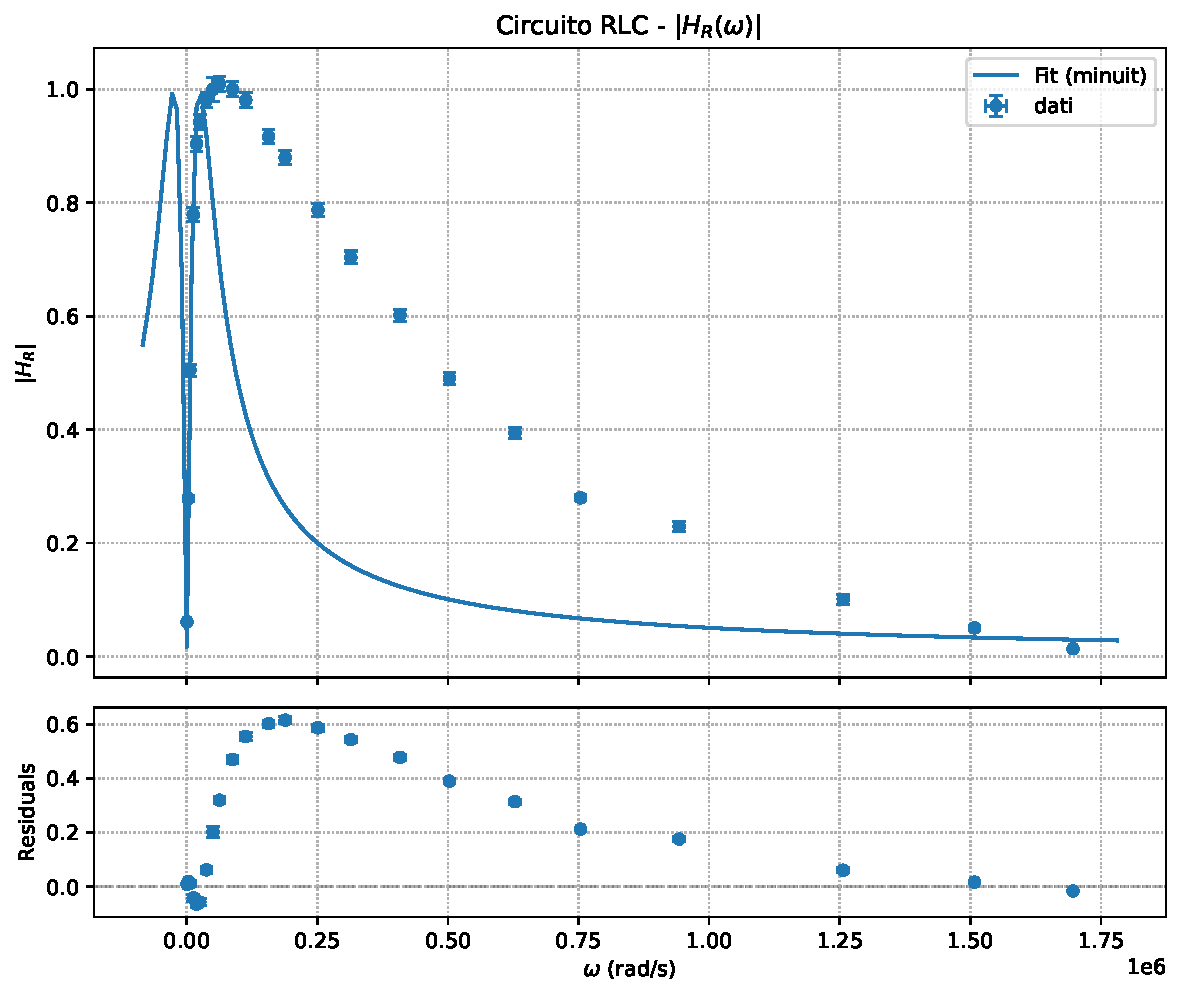
\includegraphics[width=\linewidth]{grafici/rlc_hr.pdf}
        \caption{Fit modulo $|H_R(\omega)|$ (RLC)}
        \label{fig:rlc_hr}
    \end{subfigure}
    \hfill
    \begin{subfigure}[b]{0.495\textwidth}
        \centering
        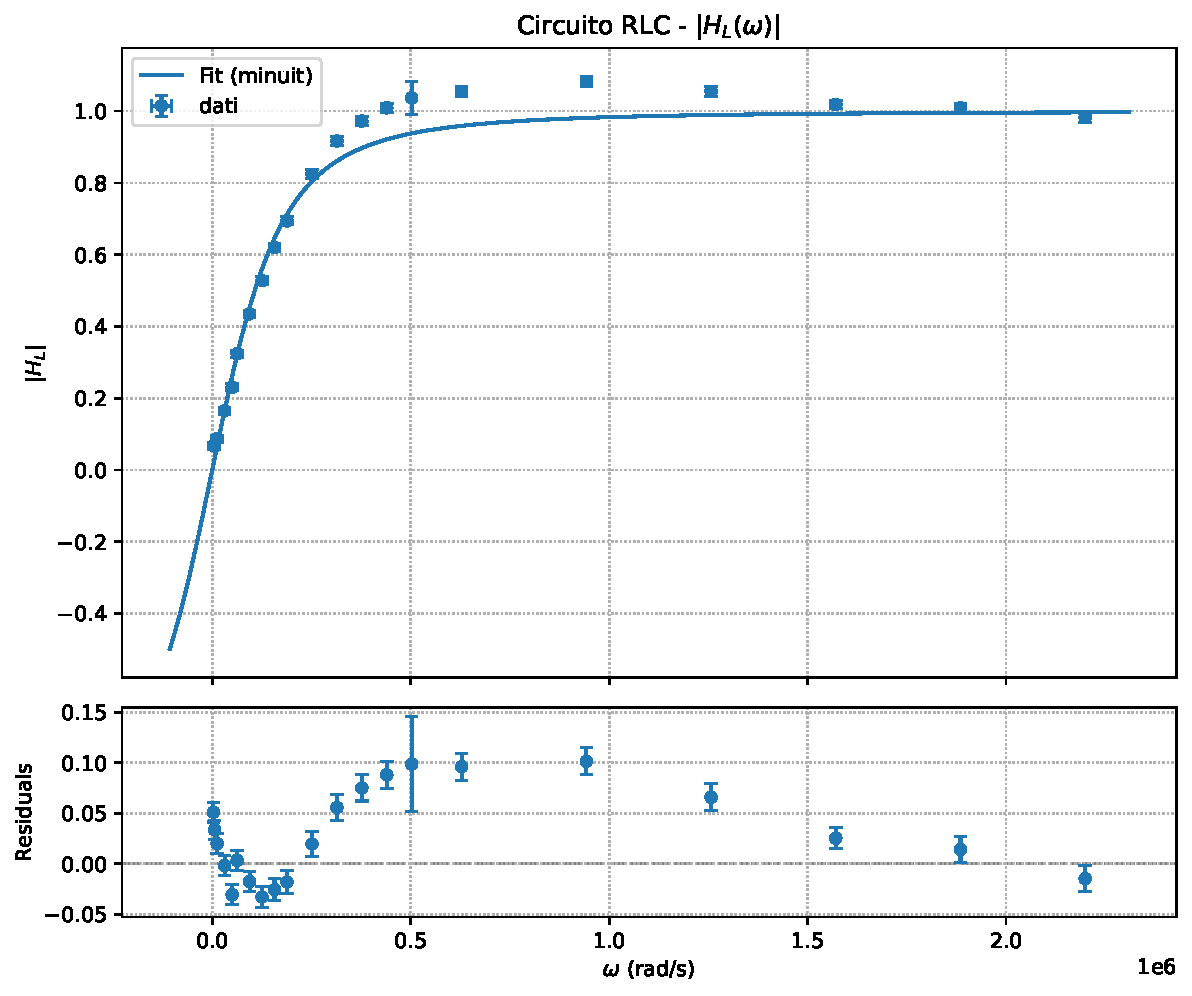
\includegraphics[width=\linewidth]{grafici/rlc_hl.pdf}
        \caption{Fit modulo $|H_L(\omega)|$ (RLC)}
        \label{fig:rlc_hl}
    \end{subfigure}

    \vspace{\baselineskip}

    \begin{subfigure}[b]{0.495\textwidth}
        \centering
        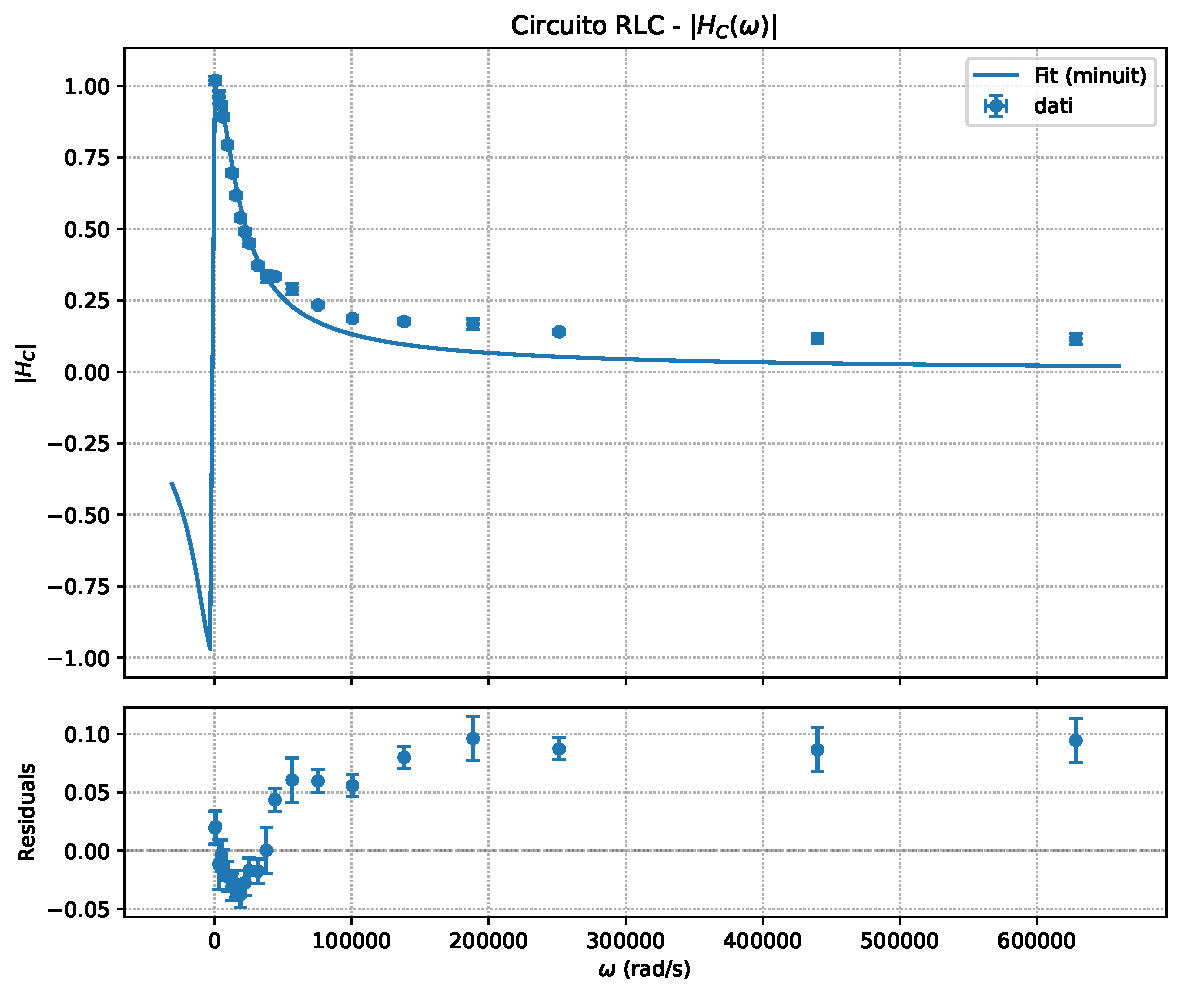
\includegraphics[width=\linewidth]{grafici/rlc_hc.pdf}
        \caption{Fit modulo $|H_C(\omega)|$ (RLC)}
        \label{fig:rlc_hc_rlc}
    \end{subfigure}
    \hfill
    \begin{subfigure}[b]{0.495\textwidth}
        \centering
        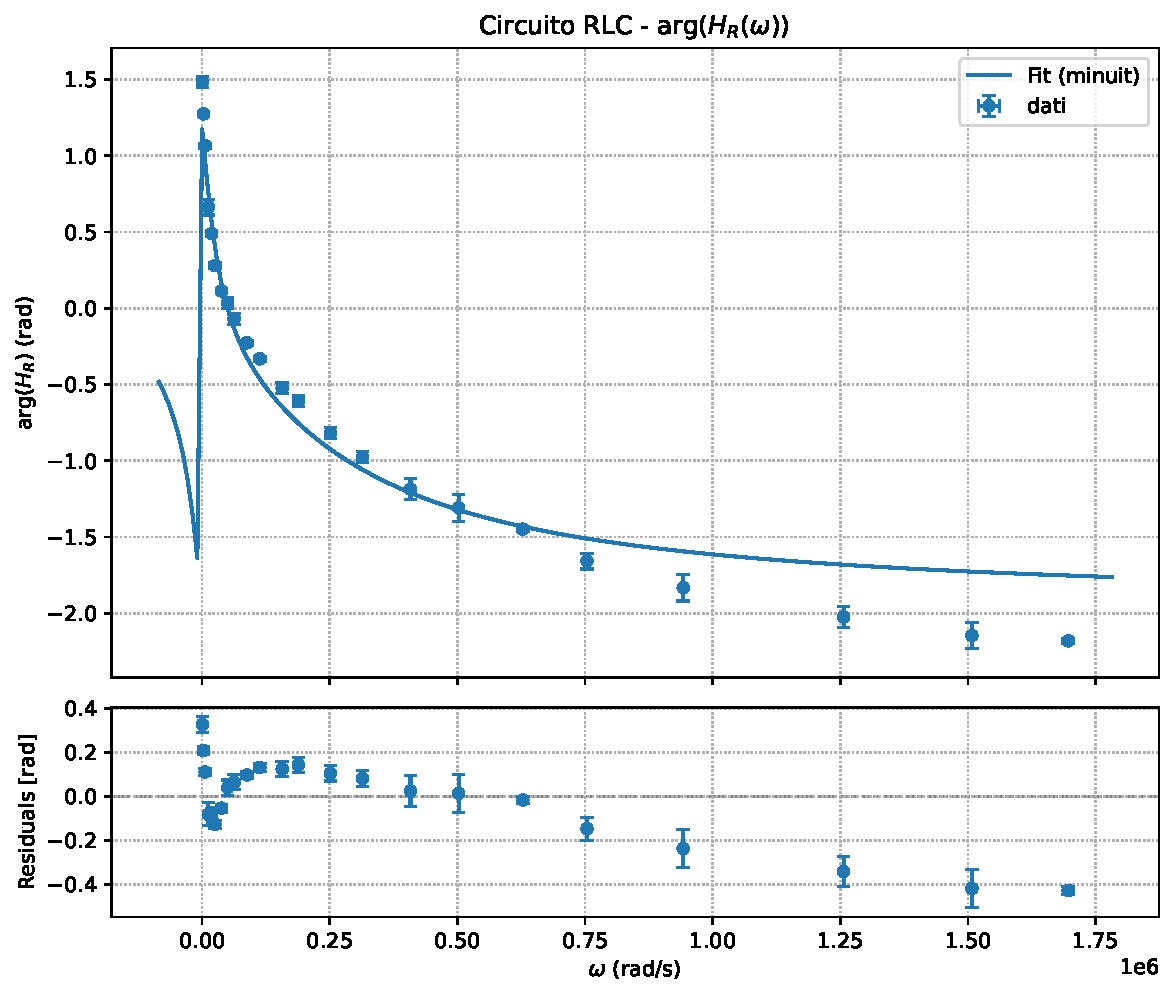
\includegraphics[width=\linewidth]{grafici/rlc_fase_hr.pdf}
        \caption{Fit fase $\arg(H_R(\omega))$ (RLC)}
        \label{fig:rlc_fase_hr}
    \end{subfigure}

    \caption{Funzioni di trasferimento per il circuito RLC (regime sovrasmorzato).}
    \label{fig:funzioni_trasferimento_rlc}
\end{figure}
Osservando la distribuzione dei dati per il modulo della funzione di trasferimento per la tensione ai capi della resistenza $|H_R(\omega)|$, essa ha un'altezza ed un'ampiezza caratteristiche. Ci aspettiamo che la funzione abbia valore massimo, pari ad 1, in corrispondenza della frequenza di risonanza, cioè per $\omega_0 = \frac{1}{\sqrt{LC}}$.
Inoltre possiamo ricavare informazioni sulla risposta in frequenza del circuito anche dalla larghezza $\Delta \omega$ della curva $|H_R(j\omega)|$. Tale larghezza corrisponde alla differenza tra le due frequenze di taglio ed è pari a $\Delta \omega = \frac{R}{L}$. Al suo aumentare, cioè all'aumentare di $R$ o al diminuire di $L$, la risposta sulla resistenza risulta meno ``selettiva''.
Il modulo di $H_R(\omega)$ infatti decrescerebbe più lentamente e si avrebbe quindi anche il passaggio di armoniche a frequenze più distanti dalla frequenza di risonanza.

L'analisi delle misure effettuate ci ha poi permesso di ricavare empiricamente i valori di capacità e induttanza, osservabili in tabella~\ref{tab:risultati_fit_rlc}.
\begin{table}[htbp]
\centering
\begin{tabular}{|l|cccc|}
\hline
Dato & $|H_R|$ & $\arg(H_R)$ & $|H_L|$ & $|H_C|$ \\\hline\hline
$L$ & 197.2 ± 1.2 mH & 27.85 ± 0.76 mH & 53.89 ± 0.61 mH & 6 ± 3000 µH \\\hline
$C$ & 8.43 ± 0.11 nF & 3.63 ± 0.12 nF & 7 ± 280 µF & 7.515 ± 0.088 nF \\\hline
$k$ & --- & -392 ± 12 mrad & --- & --- \\\hline
$\chi^2$ & 2.454e+04 & 1.16e+03 & 321 & 380 \\\hline
DoF & 21 & 20 & 19 & 20 \\\hline
$\chi^2/\nu$ & 1.17e+03 & 57.8 & 16.9 & 19 \\\hline
\end{tabular}
\caption{Risultati dei Fit per il Circuito RLC.}
\label{tab:risultati_fit_rlc}
\end{table}

Tali risultati sono stati confrontati con i valori di $C_{media}$ ($=\SI{4.40 \pm 0.06}{nF}$), proveniente dallo studio del circuito RC, e $L_{media}$ ($=\SI{51 \pm 2}{mH}$), calcolato invece in seguito all'esperienza col circuito RL. Il confronto è stato effettuato mediante t-test, il quale ci ha permesso di valutare la compatibilità tra i risultati ottenuti mediante modalità differenti. Si sono utilizzate le relazioni $ t = \frac{C_{media} - C_s}{\sqrt{\delta_{C_{media}}^2 + \delta_{C_s}^2}} $ e $ t = \frac{L_{media} - L_s}{\sqrt{\delta_{L_{media}}^2 + \delta_{L_s}^2}} $, dove ($C_s \pm \delta_{C_s}$) e ($L_s \pm \delta_{L_s}$) sono stati ricavati dai fit per il circuito RLC, mentre $\delta_{C_{media}}$ e $\delta_{L_{media}}$ indicano la deviazione standard sulla media pesata delle misure ricavate dai fit di RC e RL.
Per valutare poi la bontà dei fit effettuati abbiamo realizzato il test del chi quadro, con esiti visibili nella tabella~\ref{tab:risultati_fit_rlc}.

\subsection{Conclusione}
Basandoci sui dati ottenuti mediante il test del chi quadro (tabella~\ref{tab:risultati_fit_rlc}), possiamo affermare che le leggi attese non offrono un buon accordo con i dati ottenuti sperimentalmente, né per quanto riguarda i moduli delle varie funzioni di trasferimento né per quanto riguarda le fasi (i valori di $\chi^2/\text{DoF}$ sono molto elevati). Nonostante ciò, vale la pena osservare che in alcuni casi l'andamento dei dati campionati risulta essere qualitativamente concorde a quello della legge attesa; ovviamente tale osservazione non costituisce una prova quantitativa e attendibile della bontà della legge. Inoltre è possibile osservare che per alcuni valori di $\omega$ i valori delle funzioni di trasferimento raggiungono il valore di 1 (per $|H_R(\omega)|$) o valori significativi (per $|H_L(\omega)|$ e $|H_C(\omega)|$), e ciò accade in corrispondenza dei picchi e dunque delle frequenze di risonanza o vicino ad esse. I valori di $L$ e $C$ ricavati dalle interpolazioni non risultano compatibili con i valori ricavati nei circuiti RL e RC, ma ciò non ha una rilevanza significativa in quanto tali valori derivano da interpolazioni statisticamente non attendibili. Per lo stesso motivo non è rilevante nemmeno fare considerazioni quantitative sulle ampiezze a metà altezza delle funzioni di trasferimento.

\end{document}